%%%%%%%%%%%%%%%%%%%%%%%%%%%%%%%%%%%%%%%%%%%%%%%%%%%%%%%%%%%%%%%%%%
%
% Analysis of Algorithms
%
% Homework Assignment #6
%
%%%%%%%%%%%%%%%%%%%%%%%%%%%%%%%%%%%%%%%%%%%%%%%%%%%%%%%%%%%%%%%%%%
%%%%%%%%%%%%%%%%%%%%%%%%%%%%%%%%%%%%%%%%%%%%%%%%%%%%%%%%%%%%%%%%%%
%
% Score Card and Answer Sheets
%
%%%%%%%%%%%%%%%%%%%%%%%%%%%%%%%%%%%%%%%%%%%%%%%%%%%%%%%%%%%%%%%%%%
\documentclass[addpoints,11pt]{exam}
\usepackage{clrscode4e}
\usepackage{tcucosc}
\usepackage{units}
\usepackage{enumitem}
\usepackage{hyperref}
\usepackage{fullpage}
\usepackage{graphicx}

%%%%%%%%%%%%%%%%%%%%%%%%%%%%%%%%%%%%%%%%%%%%%%%%%%%%%%%%%%%%%%%%%%
%
% Begin Document
%
%%%%%%%%%%%%%%%%%%%%%%%%%%%%%%%%%%%%%%%%%%%%%%%%%%%%%%%%%%%%%%%%%%
\begin{document}
\pagestyle{empty}


\noindent{\large\bfseries Name: Sabyasachi Sahoo}\\
\noindent{\large\bfseries COSC 40403 - Analysis of Algorithms: Fall 2018: Homework 7}\\
\noindent{\large\bfseries Due: 23:59:59 on November 12, 2018}

%%%%%%%%%%%%%%%%%%%%%%%%%%%%%%%%%%%%%%%%%%%%%%%%%%%%%%%%%%%%%%%%%%
%
% Score Card and Answer Sheets
%
% Comment out one-or-the-other to show or not-show the answers.
%
%%%%%%%%%%%%%%%%%%%%%%%%%%%%%%%%%%%%%%%%%%%%%%%%%%%%%%%%%%%%%%%%%%
\printanswers
%%\noprintanswers


%%%%%%%%%%%%%%%%%%%%%%%%%%%%%%%%%%%%%%%%%%%%%%%%%%%%%%%%%%%%%%%%%%
%
% Score Card
%
%%%%%%%%%%%%%%%%%%%%%%%%%%%%%%%%%%%%%%%%%%%%%%%%%%%%%%%%%%%%%%%%%%
\ifprintanswers
\noindent
\begin{center}
	\gradetable[v][questions]
\end{center}
\newpage
\fi


%%%%%%%%%%%%%%%%%%%%%%%%%%%%%%%%%%%%%%%%%%%%%%%%%%%%%%%%%%%%%%%%%%
%
% Question 1
%
%%%%%%%%%%%%%%%%%%%%%%%%%%%%%%%%%%%%%%%%%%%%%%%%%%%%%%%%%%%%%%%%%%
\begin{questions}
\question[5]
Exercise 15.1-3: Consider a modification of the rod-cutting problem in which, in addition to a price $p_i$ for each rod, each cut incurs a fixed cost of $c$.  The revenue associated with a solution is now the sum of the prices of the pieces minus the costs of making the cuts.  Give a dynamic-programming algorithm to solve this modified problem.
\begin{solutionorbox} 
\\
MODIFIED-CUT-ROD(p, n, c)\\
\hspace*{5mm} let r[0..n] be a new array\\
\hspace*{5mm} r[0] = 0\\
\hspace*{5mm}  \textbf{for} j = 1 \textbf{to} n\\
\hspace*{5mm} \hspace*{5mm} q = p[j] \\
\hspace*{5mm} \hspace*{5mm} \textbf{for} i = 1 \textbf{to} j - 1\\
\hspace*{5mm} \hspace*{5mm} \hspace*{5mm} q = max(q, p[i] + r[j - i] - c)\\
\hspace*{5mm} \hspace*{5mm} r[j] = q\\
\hspace*{5mm} \textbf{return} r[n]\\

 To subtract the fixed cost from the revenue for each added cut we change the assignment to q = max(q, p[i] + r[j − i] − c). We also have to handle i.e., in the case in which we make no cuts (when i equals j). We do the assignment q = p[j] for the case of no cuts and make the loop iteration i from 1 to [j-1]. So in the case of no cuts, we won't be deducting c from the total revenue.

\end{solutionorbox}

\ifprintanswers
\newpage
\else
\bigskip
\fi


%%%%%%%%%%%%%%%%%%%%%%%%%%%%%%%%%%%%%%%%%%%%%%%%%%%%%%%%%%%%%%%%%%
%
% Question 2
%
%%%%%%%%%%%%%%%%%%%%%%%%%%%%%%%%%%%%%%%%%%%%%%%%%%%%%%%%%%%%%%%%%%
\question[5]
Exercise 15.1-4:  Modify $\proc{Memoized-Cut-Rod}$ to return not only the value but the actual solution.
\begin{solutionorbox}\\	
	Memorized-Cut-Rod-Print(p, n)\\
	let r[0..n] be a new array\\
	let s[0..n] be a new array\\
	\textbf{for} i = 0 \textbf{to} n\\
	\hspace*{5mm}r[i] = -$\infty$\\
	(val, s) = Memorized-Cut-Rod(p, n, r, s)\\
	System.out.print("The optimal value is" + val + "and the cuts are at")
	j = n\\
	while j $>$ 0\\
	\hspace*{5mm}System.out.print(s[j])\\
	\hspace*{5mm}j = j - s[j]\\
	
	Memorized-Cut-Rod(p, n, r, s)\\
	if r[n] $\geq$ 0\\
	\hspace*{5mm}\textbf{return} r[n]\\
	if n == 0\\
	\hspace*{5mm}q = 0\\
	else q = -$\infty$\\
	\hspace*{5mm}\textbf{for} i = 1 \textbf{to} n\\
	\hspace*{5mm} \hspace*{5mm} (val, s) = Memorized-Cut-Rod(p, n - i, r, s)\\
	\hspace*{5mm} \hspace*{5mm} if q < p[i] + val\\
	\hspace*{5mm} \hspace*{5mm} \hspace*{5mm} q = p[i] + val\\
	\hspace*{5mm} \hspace*{5mm} \hspace*{5mm} s[n] = i\\
	r[n] = q\\
	\textbf{return} (q, s)\\
\end{solutionorbox}

\ifprintanswers
\newpage
\else
\bigskip
\fi


%%%%%%%%%%%%%%%%%%%%%%%%%%%%%%%%%%%%%%%%%%%%%%%%%%%%%%%%%%%%%%%%%%
%
% Question 3
%
%%%%%%%%%%%%%%%%%%%%%%%%%%%%%%%%%%%%%%%%%%%%%%%%%%%%%%%%%%%%%%%%%%
\question[5]
Exercise 15.2-1: Find an optimal parenthesization of the matrix-chain product whose sequence of dimensions is: $\langle 5, 10, 3, 12, 5, 50, 6 \rangle.$ Show your work.  Use the algorithm.
\begin{solutionorbox}
\\
Using the given matrix-chain [5, 10, 3, 12, 5, 50, 6]

p0=5, p1=10, p2=3, p3=12, p4=5, p5=50, p6=6

m[i, j] = 0, if i = j,

m[i,j]= {min {m[i,k] + m[k+1, j] + pi –1pkpj}}, if i < j          



m[1,1] = m[2,2] = m[3,3] = m[4,4] = m[5,5] = m[6,6] = 0



m[1,2] = p0xp1xp2 = 5x10x3 = 150

m[2,3] = p1xp2xp3 = 10x3x12 = 360

m[3,4] = p2xp3xp4 = 3x12x5 = 180

m[4,5] = p3xp4xp5 = 12x5x50 = 3000

m[5,6] = p4xp5xp6 = 5x50x6 = 1500

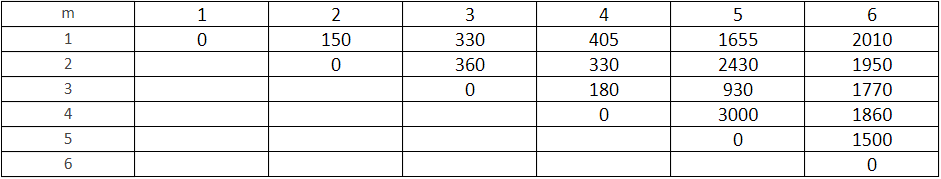
\includegraphics[scale=.75]{Image1.png}

m[i,j]= {min {m[i,k] + m[k+1, j] + pi –1pkpj}}, if i < j          
	Min of m[1,3] = 330\\
k is length of matrix\\
At k=1: m[1,3] = {min {m[1,1] + m[2,3] + p0p1p3}}  = 0 + 10x3x12 + 5x10x12 =  0+360+600= 960\\
At k= 2: m[1,3] = {min {m[1,2] + m[3,3] + p0p2p3}} = 150 + 0 + 5x3x12 = 150+0+180= 330 (min)\\

Min of m[1,4] = 405; m[2,4] = 330\\
At k=1: m[1,4] = {min {m[1,1] + m[2,4] + p0p1p4}} = 0 + 330 + 5x10x5 = 330 + 250 = 580\\
\hspace*{5mm}m[2,4] = {min {m[2,2] + m[3,4] + p1p2p4}} = 0 + 180 + 10x3x5 = 180 + 150 = 330 (min)\\
\hspace*{5mm}m[2,4] = {min {m[2,3] + m[4,4] + p2p3p4}} = 360 + 3x12x5 = 360 + 180 = 540\\
At k=2: m[1,4] = {min {m[1,2] + m[3,4] + p0p2p4}}  = 5x10x3 + 3x12x5 + 5x3x5 = 150+180+75 = 405 (min)\\
At k=3: m[1,4] = {min {m[1,3] + m[4,4] + p0p3p4}}  = 330 + 0 + 5x12x5 = 330 + 300 = 630\\

Min of m[1,5] = 1655; m[3,5] = 930; m[2,5] = 2430\\
At k=1: m[1,5] = {min {m[1,1] + m[2,5] + p0p1p5}}  = 0 + 2430 + 5x10x50 = 2430 + 2500 = 4930\\
\hspace*{5mm}For m[2,5] = {min {m[2,2] + m[3,5] + p1p2p5}} =   0 + 930 + 10x3x50 = 930 + 1500 = 2430 (min)\\
\hspace*{5mm}For m[3,5] = {min {m[3,3] + m[4,5] + p2p3p5}} = 0 + 3000 + 3x12x50 = 3000 + 1800 = 4800\\
\hspace*{5mm}For m[3,5] = {min {m[3,4] + m[5,5] + p2p4p5}} = 180 + 0 + 3x5x50 = 180 + 750 = 930 (min)\\
At k= 2: m[1,5] = {min {m[1,2] + m[3,5] + p0p2p5}} = 150 + 930 + 5x3x50 = 1080 + 750 = 1830\\
At k= 3: m[1,5] = {min {m[1,3] + m[4,5] + p0p3p5}} = 330 + 3000 + 5x12x50 = 3330 + 3000 = 6330\\
At k= 4: m[1,5] = {min {m[1,4] + m[5,5] + p0p4p5}} = 405 + 0 + 5x5x50 = 405 + 1250 = 1655 (min)\\

Min of m[1,6] = 2010; m[4,6] = 1860; m[3,6] = 1770; m[2,6] = 1950\\
At k=1: m[1,6] = {min {m[1,1] + m[2,6] + p0p1p6}}  = 0 + 1950 + 5x10x6 = 1950 + 300 = 2250\\
\hspace{5mm}For m[2,6] = {min {m[2,2] + m[3,6] + p1p2p6}} = 0 + 1770 + 10x3x6 = 1770 + 180 = 1950 (min)\\
\hspace*{5mm}For m[2,6] = {min {m[2,3] + m[4,6] + p1p3p6}} = 360 + 1860 + 10x12x6 = 2220 + 720 = 2940\\
\hspace*{5mm}For m[2,6] = {min {m[2,4] + m[5,6] + p1p4p6}} = 330 + 1500 + 10x5x6 = 1830 + 300 = 2130\\
\hspace*{5mm}For m[2,6] = {min {m[2,5] + m[6,6] + p1p5p6}} = 2430 + 0 + 10x50x6 = 2430 + 3000 = 5430\\
\hspace*{5mm}For m[3,6] = {min {m[3,3] + m[4,6] + p2p3p6}} = 0 + 1860 + 3x12x6 = 1860 + 216 = 2076 \\
\hspace*{5mm}For m[3,6] = {min {m[3,4] + m[5,6] + p2p4p6}} = 180 + 1500 + 3x5x6 = 1680 + 90 = 1770 (min)\\
\hspace*{5mm}For m[3,6] = {min {m[3,5] + m[6,6] + p2p5p6}} = 930 + 0 + 3x50x6 = 930 + 900 = 1830 \\
\hspace*{5mm}For m[4,6] = {min {m[4,4] + m[5,6] + p3p4p6}} = 0 + 1500 + 12x5x6 = 1500 + 360 = 1860 (min)\\
\hspace*{5mm}For m[4,6] = {min {m[4,5] + m[6,6] + p3p5p6}} = 3000 + 0 + 12x50x6 = 3000 + 3600 = 6600\\
At k= 2: m[1,6] = {min {m[1,2] + m[3,6] + p0p2p6}} = 150 + 1770 + 5x3x6 = 1920 + 90 = 2010 (min)\\ 
At k= 3: m[1,6] = {min {m[1,3] + m[4,6] + p0p3p6}} = 330 + 1860 + 5x12x6 = 2190 + 360 = 2550\\
At k= 4: m[1,6] = {min {m[1,4] + m[5,6] + p0p4p6}} = 405 + 1500 + 5x5x6 = 1905 + 150 = 2055\\
At k= 5: m[1,6] = {min {m[1,5] + m[6,6] + p0p5p6}} = 1655 + 0 + 5x50x6 = 1655 + 1500 = 3155\\

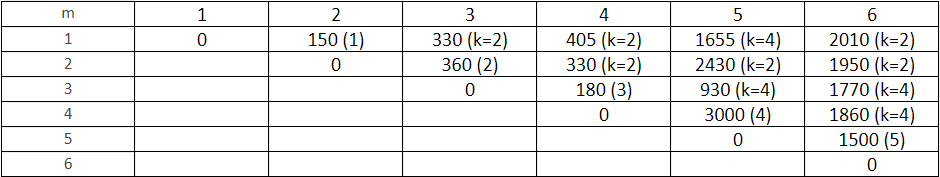
\includegraphics[scale=.75]{Image2.png}

	The required optimum multiplication order is ((A1*A2)*((A3*A4)*(A5*A6))).

\end{solutionorbox}

\ifprintanswers
\newpage
\else
\bigskip
\fi

%%%%%%%%%%%%%%%%%%%%%%%%%%%%%%%%%%%%%%%%%%%%%%%%%%%%%%%%%%%%%%%%%%
%
% Question 4
%
%%%%%%%%%%%%%%%%%%%%%%%%%%%%%%%%%%%%%%%%%%%%%%%%%%%%%%%%%%%%%%%%%%
\question[5]
Determine the LCS of $\langle 1, 0, 0, 1, 0, 1, 0, 1 \rangle$ and $\langle 0, 1, 0, 1, 1, 0, 1, 1, 0 \rangle$
\begin{solutionorbox}
	\\
	By having $\langle 1, 0, 0, 1, 0, 1, 0, 1 \rangle$ as the rows and $\langle 0, 1, 0, 1, 1, 0, 1, 1, 0 \rangle$ as the columns we get,\\
	$\begin{pmatrix}
0&0&0&0&0&0&0&0&0&0\\
0&0&1&1&1&1&1&1&1&1\\
0&1&1&2&2&2&2&2&2&2\\
0&1&1&2&2&2&3&3&3&3\\
0&1&2&2&3&3&3&4&4&4\\
0&1&2&3&3&3&4&4&4&5\\
0&1&2&3&4&4&4&5&5&5\\
0&1&2&3&4&4&5&5&5&6\\
0&1&2&3&4&5&5&6&6&6\\
\end{pmatrix}$\\

Starting from 6 at the bottom of the matrix\\
Step1- left (6),\\
Step2- left (6), \\
Step3- diagonal (6),\\
Step4- diagonal (5),\\
Step5- left (4),\\
Step6- diagonal (4),\\
Step7- diagonal (3),\\
Step8- diagonal (2),\\
Step9- up (1),\\
Step10- diagonal (6),\\
Now the diagonal values are in the set of the LCS, in the reverse of the found order.
LCS = (0,1,0,1,0,1)
\end{solutionorbox}

\ifprintanswers
\newpage
\else
\bigskip
\fi




\end{questions}
\end{document}
